% Compile with pdfLaTeX, BibTeX, then pdfLaTeX twice.
% All references are drawn from the user's master svozil.bib.
% The TikZ picture below is self-contained after copying its colour/style macros.
% Set \DistinctContextstrue for a distinct colour for each of the 16 contexts.
\documentclass[aps,pra,onecolumn,amsmath,amssymb,nofootinbib]{revtex4-2}
\usepackage{tikz}
\usetikzlibrary{calc}
\usepackage[colorlinks=true,allcolors=blue]{hyperref}
\newif\ifDistinctContexts
\DistinctContextsfalse

% Constant colours on context orbits preserve the threefold colour symmetry.
\definecolor{YOtriad}{HTML}{246A9A}
\definecolor{YObasis}{HTML}{8A939B}
\definecolor{YOspoke}{HTML}{237D70}
\definecolor{YOouterA}{HTML}{85458B}
\definecolor{YOouterB}{HTML}{B47620}
\definecolor{YOdiagonal}{HTML}{B44850}
\colorlet{YOctx1}{YOtriad}
\colorlet{YOctx2}{YOtriad}
\colorlet{YOctx3}{YOtriad}
\colorlet{YOctx4}{YObasis}
\colorlet{YOctx5}{YOspoke}
\colorlet{YOctx6}{YOspoke}
\colorlet{YOctx7}{YOspoke}
\colorlet{YOctx8}{YOouterA}
\colorlet{YOctx11}{YOouterA}
\colorlet{YOctx16}{YOouterA}
\colorlet{YOctx9}{YOouterB}
\colorlet{YOctx13}{YOouterB}
\colorlet{YOctx14}{YOouterB}
\colorlet{YOctx10}{YOdiagonal}
\colorlet{YOctx12}{YOdiagonal}
\colorlet{YOctx15}{YOdiagonal}
\ifDistinctContexts
  \definecolor{YOctx1}{HTML}{BF1FB4}
  \definecolor{YOctx2}{HTML}{B4000A}
  \definecolor{YOctx3}{HTML}{C99400}
  \definecolor{YOctx4}{HTML}{555F00}
  \definecolor{YOctx5}{HTML}{559F2A}
  \definecolor{YOctx6}{HTML}{D48A6A}
  \definecolor{YOctx7}{HTML}{F47400}
  \definecolor{YOctx8}{HTML}{B4944A}
  \definecolor{YOctx9}{HTML}{DF74BF}
  \definecolor{YOctx10}{HTML}{744ABF}
  \definecolor{YOctx11}{HTML}{35552A}
  \definecolor{YOctx12}{HTML}{C955FF}
  \definecolor{YOctx13}{HTML}{00B49F}
  \definecolor{YOctx14}{HTML}{6A558A}
  \definecolor{YOctx15}{HTML}{743F00}
  \definecolor{YOctx16}{HTML}{FF0035}
\fi
\tikzset{
  YOtrace/.style={line width=1.45pt,line cap=round,line join=round},
  YOapex/.style={line width=.68pt,line cap=round,dash pattern=on 2.4pt off 2.1pt,draw opacity=.65},
  YOlabel/.style={font=\small,inner sep=1.2pt,fill=white},
  YOnumber/.style={font=\sffamily\fontsize{8}{8}\selectfont,inner sep=0pt},
}
\newcommand{\YOline}[4]{\draw[YOtrace,YOctx#1] (v#2)--(v#3)--(v#4);}
\newcommand{\YOapexlink}[6]{%
  \draw[YOapex,draw=YOctx#1] (#3)
    -- ($(#3)!-#4!(#2)$)
    .. controls ($(#3)!-#5!(#2)$) and #6 .. (v26);%
}
\newcommand{\YOapexvia}[9]{%
  \draw[YOapex,draw=YOctx#1] (#3)
    -- ($(#3)!-#4!(#2)$)
    .. controls ($(#3)!-#5!(#2)$) and #6 .. #7
    .. controls #8 and #9 .. (v26);%
}
\newcommand{\YOvertex}[2]{%
  \foreach \context/\radius in {#2}{%
    \fill[YOctx\context] (v#1) circle[radius=\radius cm];%
  }%
  \fill[white] (v#1) circle[radius=.18cm];%
  \node[YOnumber] at (v#1) {#1};%
}

\begin{document}
\title{A Threefold-Symmetric Yu--Oh Context Diagram}
\date{\today}
\maketitle

Figure~\ref{fig:yuoh-symmetric} retains the threefold Yu--Oh layout~\cite{svozil-2025-color,Yu-2012} and the current vertex numbering. Smooth dashed curves continue the solid context lines at their endpoints, with matching tangents, to the common apex.

\begin{figure}[ht]
\centering
\resizebox{.88\linewidth}{!}{%
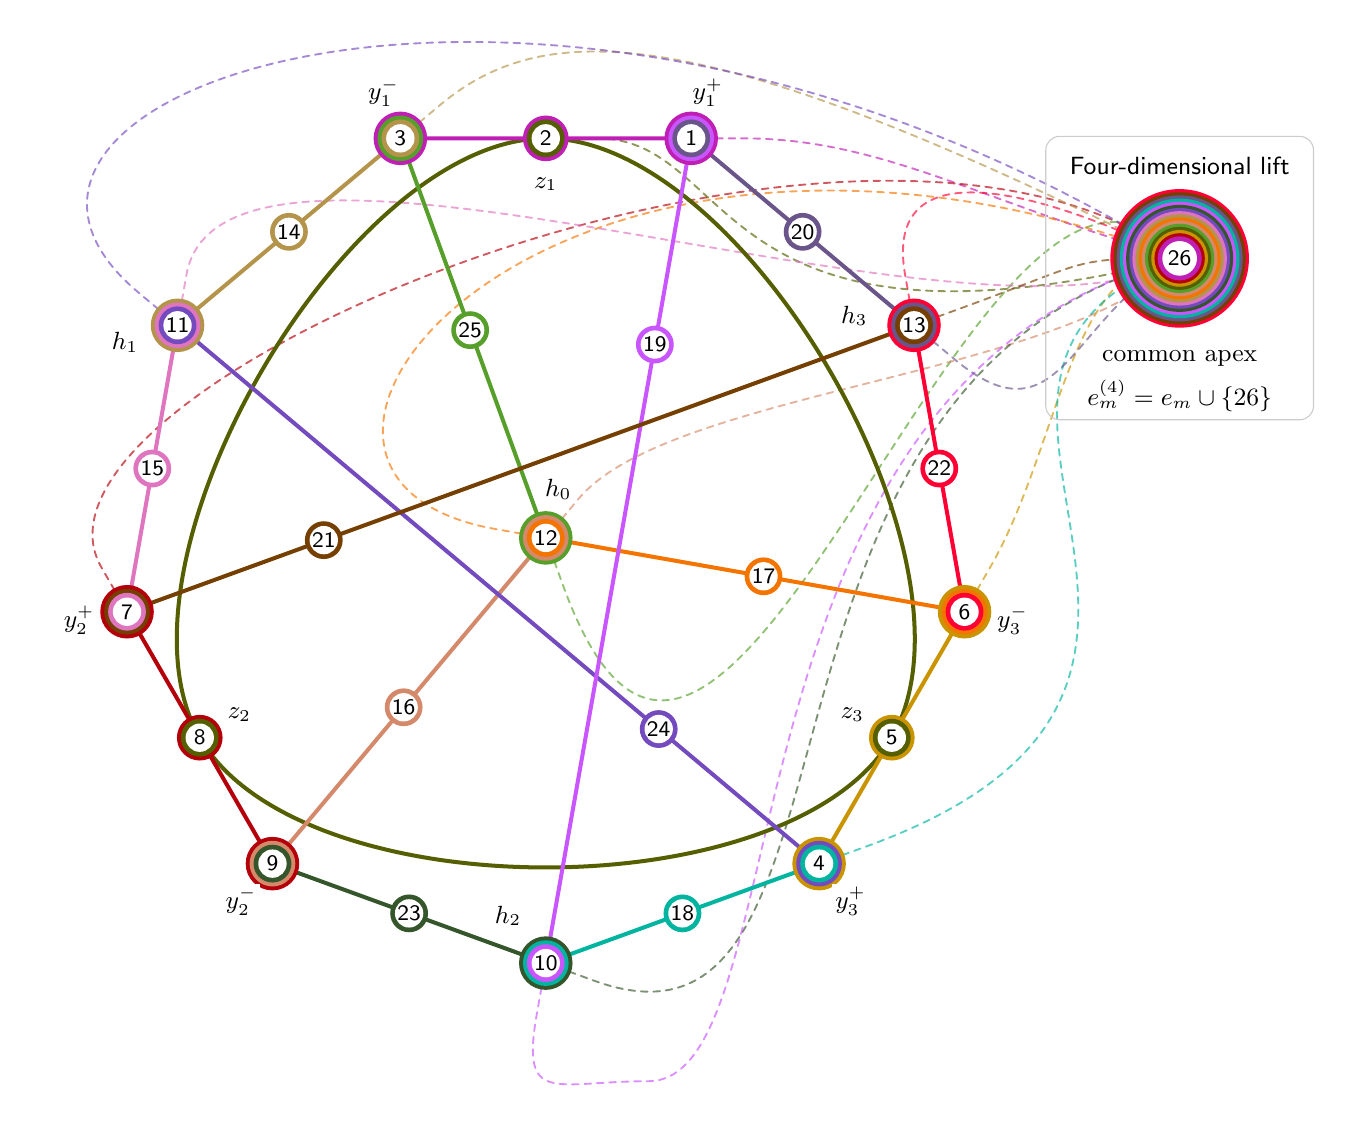
\begin{tikzpicture}[x=1cm,y=1cm]
% The nonagon is the symmetric outline of Fig. 1(a) of the earlier paper.
% Rotating by 120 degrees cycles the three coordinate directions.
\def\YOR{5.4}
\foreach \vertex/\angle in {1/70,3/110,11/150,7/190,9/230,10/270,4/310,6/350,13/30}{%
  \coordinate (v\vertex) at (\angle:\YOR);
}
\coordinate (v12) at (0,0); % h_0: fixed by the threefold rotation
% Three coordinate rays, exactly at the midpoints of the coordinate triads.
\coordinate (v2) at ($(v1)!.5!(v3)$);
\coordinate (v8) at ($(v7)!.5!(v9)$);
\coordinate (v5) at ($(v4)!.5!(v6)$);
% Six completion vertices on the outer nonagon.
\foreach \vertex/\first/\last in {14/3/11,15/11/7,23/9/10,18/10/4,22/6/13,20/13/1}{%
  \coordinate (v\vertex) at ($(v\first)!.5!(v\last)$);
}
% Three completions on the h_0 spokes.
\foreach \vertex/\last in {25/3,16/9,17/6}{%
  \coordinate (v\vertex) at ($(v12)!.52!(v\last)$);
}
% Three completions on the long chords: identical fractional positions.
\foreach \vertex/\first/\last in {24/11/4,19/10/1,21/13/7}{%
  \coordinate (v\vertex) at ($(v\first)!.75!(v\last)$);
}

% Dashed paths continue outward from terminal vertices, with exact tangency.
\coordinate (v26) at (8.05,3.55);
\coordinate (YOgrayBefore) at ($(v2)+(-1,0)$);
\YOapexlink{1}{v2}{v1}{0.351939419}{1.326540885}{(5.550000,4.250000)}
\YOapexlink{2}{v8}{v7}{0.351939419}{1.813841619}{(4.050000,6.550000)}
\YOapexlink{3}{v5}{v6}{0.351939419}{1.326540885}{(6.650000,3.550000)}
\YOapexlink{4}{YOgrayBefore}{v2}{0.650000000}{2.450000000}{(2.050000,2.050000)}
\YOapexlink{5}{v25}{v12}{0.231481481}{2.368233618}{(5.550000,6.550000)}
\YOapexlink{6}{v16}{v12}{0.231481481}{0.872507123}{(6.650000,2.050000)}
\YOapexlink{7}{v17}{v12}{0.231481481}{1.655982906}{(0.050000,6.550000)}
\YOapexlink{8}{v14}{v3}{0.351939419}{1.326540885}{(2.050000,6.550000)}
\YOapexlink{9}{v15}{v11}{0.351939419}{1.813841619}{(5.550000,2.050000)}
\YOapexlink{10}{v24}{v11}{0.081484852}{0.582930092}{(0.050000,8.550000)}
\YOapexlink{11}{v23}{v10}{0.351939419}{2.517720456}{(2.050000,2.050000)}
\YOapexvia{12}{v19}{v10}{0.081484852}{0.231918424}{(0.100000,-6.900000)}{(1.300000,-6.900000)}{(3.300000,-6.900000)}{(2.050000,2.050000)}
\YOapexlink{13}{v18}{v4}{0.351939419}{3.600610974}{(4.050000,2.050000)}
\YOapexlink{14}{v20}{v13}{0.351939419}{1.326540885}{(6.650000,2.850000)}
\YOapexlink{15}{v21}{v13}{0.081484852}{0.307135210}{(6.650000,3.550000)}
\YOapexlink{16}{v22}{v13}{0.351939419}{1.326540885}{(6.650000,4.250000)}

% Context 4: one smooth, closed threefold curve through precisely v2,v8,v5.
% Its three Bezier pieces are exact rotations of the same seed piece.
\pgfmathsetmacro{\YObasisR}{\YOR*cos(20)}
\foreach \rotation in {0,120,240}{%
  \begin{scope}[rotate=\rotation]
    \draw[YOtrace,YOctx4]
      (0,\YObasisR)
      .. controls ({-.5*\YObasisR},\YObasisR)
      and ({-(sqrt(3)/2+.25)*\YObasisR},{(-.5+.25*sqrt(3))*\YObasisR})
      .. ({-sqrt(3)/2*\YObasisR},{-.5*\YObasisR});
  \end{scope}
}
% Each solid trace is completed by its same-colour dashed connection to 26.
\YOline{1}{3}{2}{1}
\YOline{2}{9}{8}{7}
\YOline{3}{4}{5}{6}
\YOline{5}{3}{25}{12}
\YOline{6}{9}{16}{12}
\YOline{7}{6}{17}{12}
\YOline{8}{11}{14}{3}
\YOline{9}{7}{15}{11}
\YOline{10}{4}{24}{11}
\YOline{11}{9}{23}{10}
\YOline{12}{1}{19}{10}
\YOline{13}{10}{18}{4}
\YOline{14}{1}{20}{13}
\YOline{15}{7}{21}{13}
\YOline{16}{6}{22}{13}

% Nested context-colour rings, drawn after all traces.
\YOvertex{1}{1/.34,12/.29,14/.24}
\YOvertex{2}{1/.29,4/.24}
\YOvertex{3}{1/.34,5/.29,8/.24}
\YOvertex{4}{3/.34,10/.29,13/.24}
\YOvertex{5}{3/.29,4/.24}
\YOvertex{6}{3/.34,7/.29,16/.24}
\YOvertex{7}{2/.34,15/.29,9/.24}
\YOvertex{8}{2/.29,4/.24}
\YOvertex{9}{2/.34,6/.29,11/.24}
\YOvertex{10}{11/.34,13/.29,12/.24}
\YOvertex{11}{8/.34,9/.29,10/.24}
\YOvertex{12}{5/.34,6/.29,7/.24}
\YOvertex{13}{16/.34,14/.29,15/.24}
\YOvertex{14}{8/.24}
\YOvertex{15}{9/.24}
\YOvertex{16}{6/.24}
\YOvertex{17}{7/.24}
\YOvertex{18}{13/.24}
\YOvertex{19}{12/.24}
\YOvertex{20}{14/.24}
\YOvertex{21}{15/.24}
\YOvertex{22}{16/.24}
\YOvertex{23}{11/.24}
\YOvertex{24}{10/.24}
\YOvertex{25}{5/.24}

% Traditional symbols are supplementary labels; all numbers match the main paper.
\foreach \angle/\symbol in {70/{y_1^+},110/{y_1^-},190/{y_2^+},230/{y_2^-},310/{y_3^+},350/{y_3^-}}{%
  \node[YOlabel] at (\angle:6.02) {$\symbol$};
}
\node[YOlabel,anchor=east] at ($(v11)+(-.45,-.22)$) {$h_1$};
\node[YOlabel] at ($(v10)+(-.48,.60)$) {$h_2$};
\node[YOlabel] at ($(v13)+(-.76,.12)$) {$h_3$};
\foreach \angle/\symbol in {90/{z_1},210/{z_2},330/{z_3}}{%
  \node[YOlabel] at (\angle:{\YObasisR-.58}) {$\symbol$};
}
\node[YOlabel] at (.16,.62) {$h_0$};

% Common apex: dashed context continuations meet underneath these rings.
\draw[draw=black!20,rounded corners=5pt] (6.35,1.50) rectangle (9.75,5.10);
\node[font=\sffamily\small] at (8.05,4.72) {Four-dimensional lift};
\foreach \context/\radius in {16/.88,15/.84,14/.80,13/.76,12/.72,11/.68,10/.64,9/.60,8/.56,7/.52,6/.48,5/.44,4/.40,3/.36,2/.32,1/.28}{%
  \fill[YOctx\context] (v26) circle[radius=\radius cm];
}
\fill[white] (v26) circle[radius=.22cm];
\node[YOnumber] at (v26) {26};
\node[font=\small] at (8.05,2.28) {common apex};
\node[font=\small] at (8.05,1.80) {$e_m^{(4)}=e_m\cup\{26\}$};
% Use the visible curve extents, excluding distant Bezier control handles.
\pgfresetboundingbox
\path[use as bounding box] (-6.580000,-7.120032) rectangle (10.080000,6.480000);
\end{tikzpicture}%
}
\caption{Yu--Oh context diagram and its apex suspension. The base has $25$ vertices and $16$ three-element contexts. Each dashed curve leaves the end of its straight context trace with the same outward tangent and joins apex $26$, displaying a four-element context. The grey coordinate context $\{2,5,8\}$ joins the apex tangentially at vertex $2$. Unmarked crossings are not vertices. Colours identify the six context orbits under the $120^\circ$ rotation; rings record incident context colours. Traditional symbols label the original $13$ rays.}\label{fig:yuoh-symmetric}
\end{figure}

The $120^\circ$ rotation fixes $12=h_0$ and cycles the remaining base vertices in eight triples. On context indices it acts as $(1\ 2\ 3)(5\ 6\ 7)(8\ 11\ 16)(9\ 13\ 14)(10\ 12\ 15)$, with context $4$ fixed. The dashed continuations record the membership of the fixed apex $26$ in every context; the base geometry and its colour symmetry are unchanged.

\bibliography{svozil}
\end{document}
